\section{Orchestra Manager}\label{orchestraManager}

Orchestra Manager

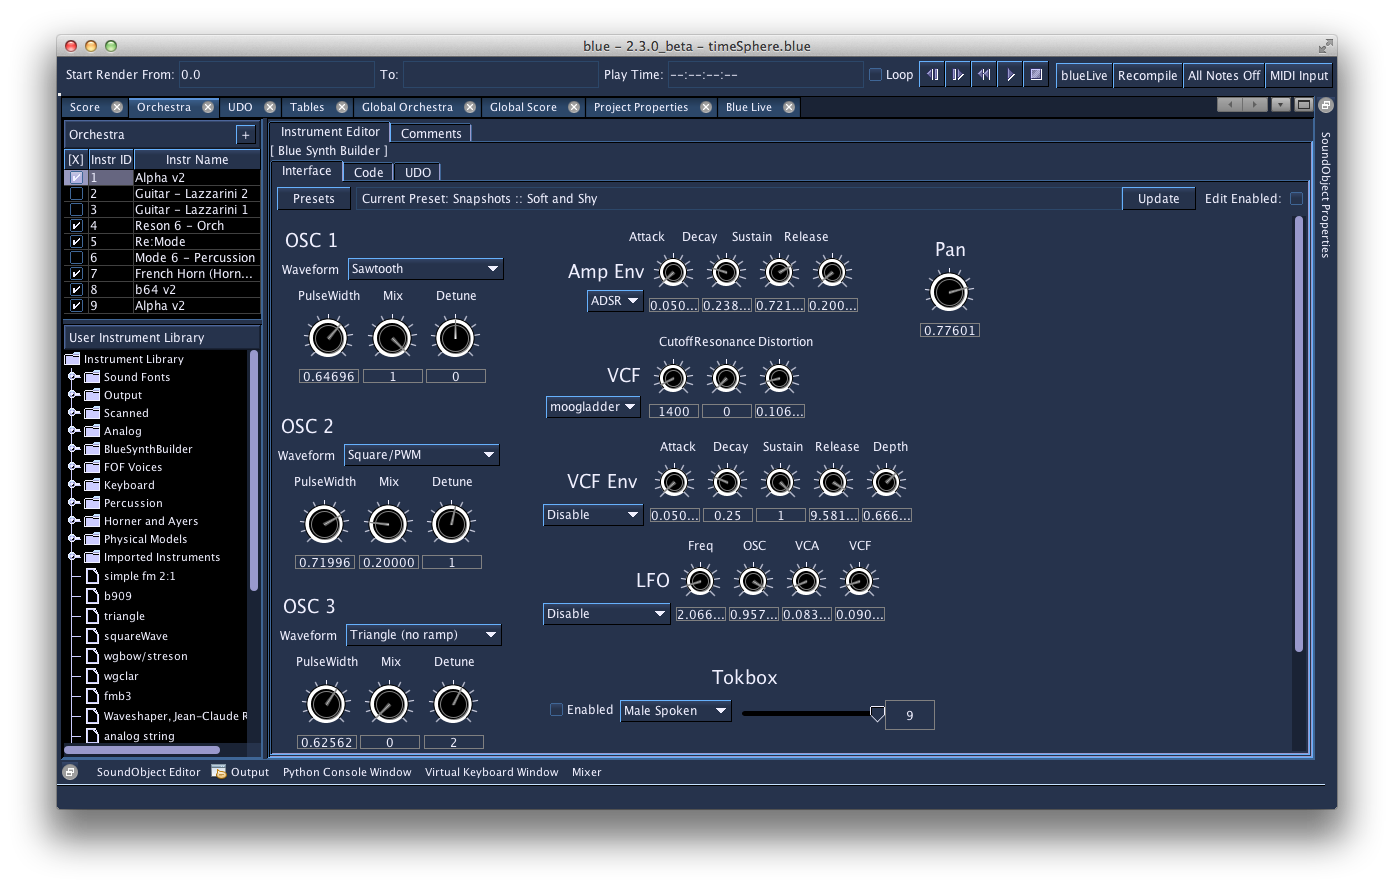
\includegraphics[width=1.00000\textwidth]{images/orchestra.png}

The Orchestra Manager is where the user organizes and edits the
orchestra for the project as well as their user Instrument Library.

In the User Instrument Library (the tree pictured on the left), you can
create instruments as well as categorize them into groups. Most actions
in this editor are accessible by right clicking with the mouse to access
popup menus. (keyboard shortcuts of ctrl-x, ctrl-c, and ctrl-v work for
cutting, copying, and pasting nodes of the tree). To edit the name of
Instruments or Groups, double click the name in the tree or hilight the
node and press F2. This library of instruments is available across
projects and is useful for building up and organizing a personal
instrument library.

To copy instruments into the library from the project's Orchestra, you
can drag and drop the instrument on the library tree to make a copy of
the instrument. To copy an instrument from the Library to the project's
orchestra, you can similarly drag and drop an instrument from the
Library to the Orchestra. You may also use cut/copy/paste to move
instrument from one to the other.

The Orchestra panel (located in the top left of the picture) is where
you will place your instruments to be used for your project. The "+"
button allows you to create new instruments from one of the available
Blue instrument types. You can also right-click on the Orchestra to show
options for copying/pasting. Once instruments are in the Orchestra, you
can edit what their instrument ID's: these may be either numbers or
strings (i.e. 3 for "instr 3", violin for "instr violin"). Selecting an
instrument will show its editor in the Instrument editor section on the
right.

On the right hand side of the Orchestra Manager is the area for editing
instruments. To make more space available for editing an instrument, you
can drag the split pane splitter to the left, or double-click the
splitter to have it collapse to the left-hand side. Each blue
instrument-type has its own editor. Note: if you are editing and
instrument from the Library, blue will show a green border with the
title "Editing Library Instrument" to help notify you what instrument
you are editing.

For projects before 0.94.0, imported projects will have their
instruments largely setup in the same way as they were before.

For projects that were in the 0.94.0 beta series, per-project Instrument
Libraries will be removed. An option to import the instrument library
will be presented to the user and if the user agrees, a folder entitled
"Imported from Project" will be added to the root of the user's
InstrumentLibrary. On the whole, it is recommended to import the
library, review the instruments, and simply remove what is not
necessary. Deleting the imported library is as simple as deleting the
folder for the imported group. Instruments in these project's
Arrangements will be modified to hold copies of the instruments from the
library as opposed to being references to instrument in the library.
(Previously, if two instruments in the Arrangement pointed to the same
instrument in the per-project InstrumentLibrary, changes to the
instrument in the library would affect all instruments in the Arrangment
that pointed to it. Now, only copies are made and no references are
used.)
